\documentclass[11pt]{article}
\usepackage{my_syllabus}
\begin{document}
\begin{figure}
\includegraphics[width=1in]{madscientistmuppet}\includegraphics[width=2in]{UVU_Horizontal_Mark_1-color}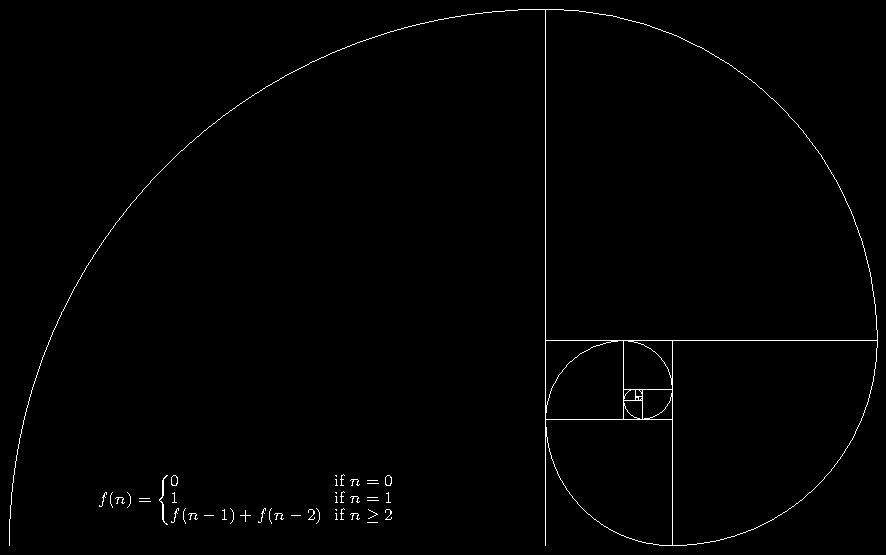
\includegraphics[width=2in]{fibonacci-spiral}\includegraphics[width=1in]{Rplot001}
\end{figure}



   \begin{center}

     {\bighelv ENG 2020 Intermediate Composition - Spring 2010} \\
     {\mediumhelv Science \& Technology Research} \\
     \ \\
     \ \\

     \begin{tabular}{ l r }

       \begin{tabular}{l}
          Instructor: Joshua Bowles      \\                                             
          Office: none                    \\                                                  
          E-mail: uvucompbowles@gmail.com  \\                                               
	  Website: \href{http://sites.google.com/site/scitechcompositionandresearch/}{http://sites.google.com/site/scitechcompositionandresearch/}\\
          Blog: \href{http://linguisticlogic.wordpress.com/}{Linguistic Logic}\\
\\ 
\\     
 \end{tabular}

       &

       \begin{tabular}{l}
          Class: MWF \\
          Office Hours: By appointment only \\ 
	  \textbf{I do NOT use my UVU e-mail} \\ 
            {}                                 \\
            {}                                  \\
          %\phantom{Office Hours:} By appointment                \\                                               
                                            \\        
                                            \\                                     
       \end{tabular}

     \end{tabular}

   \end{center}
   \ \\


   {\bf Textbooks}\\
{\bf \textsl {A\&B}}: Ramage, John D., and John C. Bean, and June Johnson. {\sl The Allyn and Bacon Guide to 
Writing}. 5th edition. New York: Pearson Longman, 2009. ISBN-13:978-0-205-59873-1. 
(A link for used versions:  \href{http://www.amazon.com/Allyn-Bacon-Guide-Writing-MyCompLab/dp/0205598730/ref=sr
_1_3/175-1452668-8158623?ie=UTF8&s=books&qid=1245772101&sr=1-3}{here}.) \\
{\bf \textsl {DK}}: Wysocki, Anne Frances, and Dennis A. Lynch. {\sl The DK Handbook.} New York: Pearson Longman, 
2008. ISBN-13 978-0-321-42053-4. 
   \ \\

   {\bf Course Outline and Grades}\\
   We will focus on methods of analyzing ideas and how to communicate such methods (and their results) in written form. You will demonstrate your ability to think in written form (and your development) through the following:
   \begin{enumerate}
     \item Informative \& Surprising, 4-6 pgs
     \item Analysis \& Synthesis, 4-6 pgs
     \item Abstract \& Annotated Bibliography, 3 pgs
     \item Final: Classical Argument, 10-12 pgs
     \item A number of responses
   \end{enumerate}

The breakdown of grades and letter grade assignment will be according to the following:
\vskip 2mm
  
\begin{tabular}{|l|l|}
\hline
Attendance & 15\\
Responses & 15\\
3 Short Papers & 45\\
1 Final Paper & 20\\
Portfolio & 5\\
\hline
\end{tabular} \  \  \  \  \ \begin{tabular}{|l|l|}
   \hline
   93-100 gives A &  73-76 gives C\\
   90-92 gives A- & 70-72 gives C-\\
   87-89 gives B+ & 67-69 gives D+\\
   83-86 gives B & 63-66 gives D\\
   80-82 gives B- & 60-62 gives D-\\
   79-77 gives C+ & 00-59 gives E\\
   \hline 
   \end{tabular}
   \ \\


 \includegraphics[width=0.1\textwidth]{Rplot003}\includegraphics[width=0.1\textwidth]{Rplot002} \quad \textcolor{teal}{{\sc Focus of this class}} \quad \includegraphics[width=0.1\textwidth]{Rplot004}\includegraphics[width=0.1\textwidth]{Rplot005}\\ 
       
The focus of this class is primarily on research that you will be directing yourself. This means that you need to develop a research agenda in conjunction with the course outline and goals. There is plenty of time given at the beginning of the semester to help you find an appropriate topic and develop a strategic course of action. Additionally, I pick some kind of topic (that I am currently working on) to address throughout the course. This gives some stability and consistency to course lectures and assignments, but \textcolor{blue}{does NOT mean you have to do your research project on this topic}. This semester we will be focusing on statistics and media (and I will be using various tools from the statistical programming language R that may be used for demonstration). Things of the nature: \texttt{the number of children shot with guns doubles every year; 5\% of football players will get dimentia; you have 30\% chance of dying}.\footnote{These are fake stats.} No knowledge of statistics (or R) is needed.
\paragraph{Comment}  
You should find something that engages you. Even topics you think might not be ``allowed'' for a college paper (e.g., I have had students write about such varied things as time-travel, medieval knights, Mayan calender, alien life, \textsl{et cetera}). The point of attending University is to get the chance to have a \emph{transformative experience}. You can have a good experience in this class, and do interesting research, if you pick topics that are really cool.\\ 
\ \\
 {\bf Portfolio}\\
   Save {\bf ALL} written assignments in this class. I elaborate on this as the semester proceeds.
  \\ 

   {\bf Notes on the Calendar and Organization}\\
   \textcolor{red}{ATTENDANCE IS MANDATORY}. As the course proceeds we usually change the schedule. I say {\it we} because I take input from students seriously. However, if you miss class you miss the chance to help shape the class, and more importantly, you miss changes to the schedule. The overall structure and timeline of the class is always maintained, but we are also very flexible and dynamic because we are sensitive to current media and science events. If you miss class, you miss this dynamic progression. It is your responsibility to find out any information you miss.
   \\ 
       

   {\bf Academic Integrity}\\
 Cheating, plagiarism, or any unethical academic behavior is not tolerated. It will be reported immediately to 
your Major Department and Student Services. See plagiarism policy 
\href{http://www.uvu.edu/english/student/plagiarism.html}{here} or at http://www.uvu.edu/english/student/
plagiarism.html.
 \\
  
  
  {\bf UVU Resources}\\
  The following is a list (with active links) of some basic research corpora.
  \begin{enumerate}
\item UVU library: \href{http://www.uvu.edu/library}{http://www.uvu.edu/library}
\item Library search engines: \href{http://www.uvu.edu/library/search/index.php}
{http://www.uvu.edu/library/search/index.php}
\item UVU writing center: \href{http://www.uvsc.edu/owl}{http://www.uvsc.edu/owl}
\end{enumerate}

% \documentclass[11pt]{article}
% 
% \usepackage[usenames]{xcolor}
% 
% 
% \begin{document}
% \author{Joshua Bowles}
% \title{Eng 2020 Spring 2010 Schedule}
% \date{January, 14 2010}
% 
% 
% \maketitle

   {\bf The schedule here is {\it tentative} and will most likely be modified. It is your responsibility to keep track of the changes as I announce them in class.}\\
   \begin{enumerate}
\item JAN 6 W: (week 1): Introductions; find syllabus, register UV link and e-mail; \textbf{Read Blog; Scholar I}
\item[] JAN 8 F: Open discussion
\item  JAN 11 M (week 2): Mathematical Induction and Rational Inference 
\item[] JAN 13 W: \textcolor{red}{\texttt{Blog Response DUE;}} Lecture on convention and language  
\item[] JAN 15 F: Research questions A\&B:243-5; A\&B:579, 602-4

\item  JAN 18 M (week 3): \textcolor{magenta}{MARTIN LUTHER KING JR. DAY}
\item[] JAN 20 W: Mathematical Symmetry ({\sl Illuminated} video); Thesis statement\ldots bring on Friday; \textbf{Read DK:102-3,146-7.}
\item[] JAN 22 F: EXERCISE---A\&B:223\ldots work on extending thesis statement; \textbf{Read DK:102-113}

\item  JAN 25 M (week 4): Begin paper \#1: formats, questions, thesis statements; Mathematical Probability ({\sl Illuminated} video)
\item[] JAN 27 W: What is evidence? DEMO---Python {\sl Genesis, Innaguaral, Chat}: Evidence to support thesis statements; \textbf{Read A\&B:41-47}
\item[] JAN 29 F: Essay \#1 peer review (1st); \textcolor{red}{\texttt{Scholar I Response DUE}} 

\item FEB 1 M (week 5): What is evidence? Ranking Evidence Types; Mathematical Probability ({\sl Illuminated} video)
\item[] FEB 3 W: Essay \#1 peer review (2nd)
\item[] FEB 5 F: \textcolor{olive}{Library Day---Research/Writing}

\item FEB 8 M (week 6): \textcolor{red}{\texttt{\#1 Informative and Surprising (4-6 pgs) DUE;}} What is Analysis/Synthesis; \textcolor{teal}{{\sc find two articles for Essay \#2}}; \textbf{Read DK:88-96} 
\item[] FEB 10 W: What is Rhetoric? EXERCISE---A\&B:350 1-6; {\bf Read A\&B ch. 13, DK:2-13}
\item[] FEB 12 F: Essay \#2 peer review (1st) 

\item FEB 15 M (week 7): \textcolor{magenta}{PRESIDENT'S DAY}
\item[] FEB 17 W: DEMO---``Computational'' Rhetoric and Statistics
\item[] FEB 19 F: Essay \#2 peer review (2nd); \textcolor{red}{\texttt{Summaries to research articles (2 pgs; 1 per article) DUE}}

\item FEB 22 M (Week 8): \textcolor{olive}{Writing Day}
\item[] FEB 24 W: Workshop on analysis and generating ideas for rhetorical strategies--A\&B:362
\item[]  FEB 26 F: \textcolor{red}{\texttt{\#2 Analysis and Synthesis (4-6 pgs) DUE}}; Read \textsl{TSIS} Chapter 4

\item MARCH 1 M (week 9): Proposals, Abstracts, Annotated Bibliographies; Read {\sl TSIS} Chapter 5
\item[] MARCH 3 W: Draft proposals/abstracts
\item[] MARCH 5 F: Meet in Library; {\bf Look over DK:18-87, 360}; Read {\sl TSIS} Chapters 2, 3

\item MARCH 8 M (week 10): \textcolor{olive}{Library day DO YOUR RESEARCH!!}
\item[] MARCH 10 W: \textcolor{red}{\texttt{\#3 Abstract (1 pg) and Annotated Bibliography DUE}}; {\bf Read A\&B ch. 14}, {\sl TSIS} Chapters 6, 7
\item[] MARCH 12 F: Essay\#4 peer review (1st); start making presentations (use \#4 draft as guideline)

\item MARCH 15 M (week 11): DEMO---Coprora results on {\sl TSIS}; Research Presentations (5-10 minutes) 
\item[] MARCH 17 W: \textcolor{magenta}{SPRING BREAK}, begins on 16th
\item[] MARCH 19 F: \textcolor{magenta}{SPRING BREAK}

\item MARCH 22 M (week 12): Research Presentations (5-10 minutes)
\item[] MARCH 24 W: Research Presentations (5-10 minutes)
\item[] MARCH 26 F: Research Presentations (5-10 minutes); \textcolor{red}{\texttt{Response Y DUE}}

\item MARCH 29 M (week 13): Light Week: Research Presentations (5-10 minutes)
\item[] MARCH 31 W: \#4 peer review (2nd)
\item[] APRIL 2 F: \#4 peer review (2.2nd)

\item APRIL 5 M (week 14): Syllogistic Logic; Read {\sl TSIS} Part 3---(Chapters 8, 9, 10)
\item[] APRIL 7 W: Syllogisms and Fallacies
\item[] APRIL 9 F: Inference and Pressuposition; \textcolor{red}{\texttt{Response Z DUE}}

\item APRIL 12 M (week 15): Essay \#4 peer review (3rd); directions for \textcolor{blue}{Portfolio}
\item[] APRIL 14 W: Workshop---supporting claims with evidence
\item[] APRIL 16 F: Workshop---style, voice, audience

\item APRIL 19 M (week 16): Essay \#4 peer review (4th and last one)
\item[] APRIL 21 W:  Open discussion about logic, style, voice, audience---will accept Portfolios
\item[] APRIL 23 F: STUDY DAY

\item APRIL 26 M (FINALS WEEK!!): open
\item[] APRIL 28 W: \textcolor{red}{\texttt{Portfolio, Classical Argument (10-12pgs) DUE}}
\item[] APRIL 29 F: \textcolor{green}{FALL 2009 SEMESTER ENDS}
\end{enumerate}

% \end{document}

\end{document}

